
%% bare_jrnl.tex
%% V1.3
%% 2007/01/11
%% by Michael Shell
%% see http://www.michaelshell.org/
%% for current contact information.
%%
%% This is a skeleton file demonstrating the use of IEEEtran.cls
%% (requires IEEEtran.cls version 1.7 or later) with an IEEE journal paper.
%%
%% Support sites:
%% http://www.michaelshell.org/tex/ieeetran/
%% http://www.ctan.org/tex-archive/macros/latex/contrib/IEEEtran/
%% and
%% http://www.ieee.org/



% *** Authors should verify (and, if needed, correct) their LaTeX system  ***
% *** with the testflow diagnostic prior to trusting their LaTeX platform ***
% *** with production work. IEEE's font choices can trigger bugs that do  ***
% *** not appear when using other class files.                            ***
% The testflow support page is at:
% http://www.michaelshell.org/tex/testflow/


%%*************************************************************************
%% Legal Notice:
%% This code is offered as-is without any warranty either expressed or
%% implied; without even the implied warranty of MERCHANTABILITY or
%% FITNESS FOR A PARTICULAR PURPOSE! 
%% User assumes all risk.
%% In no event shall IEEE or any contributor to this code be liable for
%% any damages or losses, including, but not limited to, incidental,
%% consequential, or any other damages, resulting from the use or misuse
%% of any information contained here.
%%
%% All comments are the opinions of their respective authors and are not
%% necessarily endorsed by the IEEE.
%%
%% This work is distributed under the LaTeX Project Public License (LPPL)
%% ( http://www.latex-project.org/ ) version 1.3, and may be freely used,
%% distributed and modified. A copy of the LPPL, version 1.3, is included
%% in the base LaTeX documentation of all distributions of LaTeX released
%% 2003/12/01 or later.
%% Retain all contribution notices and credits.
%% ** Modified files should be clearly indicated as such, including  **
%% ** renaming them and changing author support contact information. **
%%
%% File list of work: IEEEtran.cls, IEEEtran_HOWTO.pdf, bare_adv.tex,
%%                    bare_conf.tex, bare_jrnl.tex, bare_jrnl_compsoc.tex
%%*************************************************************************

% Note that the a4paper option is mainly intended so that authors in
% countries using A4 can easily print to A4 and see how their papers will
% look in print - the typesetting of the document will not typically be
% affected with changes in paper size (but the bottom and side margins will).
% Use the testflow package mentioned above to verify correct handling of
% both paper sizes by the user's LaTeX system.
%
% Also note that the "draftcls" or "draftclsnofoot", not "draft", option
% should be used if it is desired that the figures are to be displayed in
% draft mode.
%
\documentclass[draftclsnofoot,12pt,journal,onecolumn]{IEEEtran}
\renewcommand{\rmdefault}{phv} % Arial
\renewcommand{\sfdefault}{phv} % Arial
\setcounter{page}{3}

%
% If IEEEtran.cls has not been installed into the LaTeX system files,
% manually specify the path to it like:
% \documentclass[journal]{../sty/IEEEtran}





% Some very useful LaTeX packages include:
% (uncomment the ones you want to load)


% *** MISC UTILITY PACKAGES ***
%
\usepackage{ifpdf}
% Heiko Oberdiek's ifpdf.sty is very useful if you need conditional
% compilation based on whether the output is pdf or dvi.
% usage:
% \ifpdf
%   % pdf code
% \else
%   % dvi code
% \fi
% The latest version of ifpdf.sty can be obtained from:
% http://www.ctan.org/tex-archive/macros/latex/contrib/oberdiek/
% Also, note that IEEEtran.cls V1.7 and later provides a builtin
% \ifCLASSINFOpdf conditional that works the same way.
% When switching from latex to pdflatex and vice-versa, the compiler may
% have to be run twice to clear warning/error messages.






% *** CITATION PACKAGES ***
%
\usepackage{cite}
% cite.sty was written by Donald Arseneau
% V1.6 and later of IEEEtran pre-defines the format of the cite.sty package
% \cite{} output to follow that of IEEE. Loading the cite package will
% result in citation numbers being automatically sorted and properly
% "compressed/ranged". e.g., [1], [9], [2], [7], [5], [6] without using
% cite.sty will become [1], [2], [5]--[7], [9] using cite.sty. cite.sty's
% \cite will automatically add leading space, if needed. Use cite.sty's
% noadjust option (cite.sty V3.8 and later) if you want to turn this off.
% cite.sty is already installed on most LaTeX systems. Be sure and use
% version 4.0 (2003-05-27) and later if using hyperref.sty. cite.sty does
% not currently provide for hyperlinked citations.
% The latest version can be obtained at:
% http://www.ctan.org/tex-archive/macros/latex/contrib/cite/
% The documentation is contained in the cite.sty file itself.



%\usepackage{hyperref}


% *** GRAPHICS RELATED PACKAGES ***
%
\ifCLASSINFOpdf
  % \usepackage[pdftex]{graphicx}
  % declare the path(s) where your graphic files are
  % \graphicspath{{../pdf/}{../jpeg/}}
  % and their extensions so you won't have to specify these with
  % every instance of \includegraphics
  % \DeclareGraphicsExtensions{.pdf,.jpeg,.png}
\else
  % or other class option (dvipsone, dvipdf, if not using dvips). graphicx
  % will default to the driver specified in the system graphics.cfg if no
  % driver is specified.
   \usepackage[dvips]{graphicx}
  % declare the path(s) where your graphic files are
   \graphicspath{{../figures/}}
  % and their extensions so you won't have to specify these with
  % every instance of \includegraphics
  % \DeclareGraphicsExtensions{.eps}
\fi
% graphicx was written by David Carlisle and Sebastian Rahtz. It is
% required if you want graphics, photos, etc. graphicx.sty is already
% installed on most LaTeX systems. The latest version and documentation can
% be obtained at: 
% http://www.ctan.org/tex-archive/macros/latex/required/graphics/
% Another good source of documentation is "Using Imported Graphics in
% LaTeX2e" by Keith Reckdahl which can be found as epslatex.ps or
% epslatex.pdf at: http://www.ctan.org/tex-archive/info/
%
% latex, and pdflatex in dvi mode, support graphics in encapsulated
% postscript (.eps) format. pdflatex in pdf mode supports graphics
% in .pdf, .jpeg, .png and .mps (metapost) formats. Users should ensure
% that all non-photo figures use a vector format (.eps, .pdf, .mps) and
% not a bitmapped formats (.jpeg, .png). IEEE frowns on bitmapped formats
% which can result in "jaggedy"/blurry rendering of lines and letters as
% well as large increases in file sizes.
%
% You can find documentation about the pdfTeX application at:
% http://www.tug.org/applications/pdftex





% *** MATH PACKAGES ***
%
\usepackage[cmex10]{amsmath}
\usepackage{amsfonts}
% A popular package from the American Mathematical Society that provides
% many useful and powerful commands for dealing with mathematics. If using
% it, be sure to load this package with the cmex10 option to ensure that
% only type 1 fonts will utilized at all point sizes. Without this option,
% it is possible that some math symbols, particularly those within
% footnotes, will be rendered in bitmap form which will result in a
% document that can not be IEEE Xplore compliant!
%
% Also, note that the amsmath package sets \interdisplaylinepenalty to 10000
% thus preventing page breaks from occurring within multiline equations. Use:
%\interdisplaylinepenalty=2500
% after loading amsmath to restore such page breaks as IEEEtran.cls normally
% does. amsmath.sty is already installed on most LaTeX systems. The latest
% version and documentation can be obtained at:
% http://www.ctan.org/tex-archive/macros/latex/required/amslatex/math/





% *** SPECIALIZED LIST PACKAGES ***
%
%\usepackage{algorithmic}
% algorithmic.sty was written by Peter Williams and Rogerio Brito.
% This package provides an algorithmic environment fo describing algorithms.
% You can use the algorithmic environment in-text or within a figure
% environment to provide for a floating algorithm. Do NOT use the algorithm
% floating environment provided by algorithm.sty (by the same authors) or
% algorithm2e.sty (by Christophe Fiorio) as IEEE does not use dedicated
% algorithm float types and packages that provide these will not provide
% correct IEEE style captions. The latest version and documentation of
% algorithmic.sty can be obtained at:
% http://www.ctan.org/tex-archive/macros/latex/contrib/algorithms/
% There is also a support site at:
% http://algorithms.berlios.de/index.html
% Also of interest may be the (relatively newer and more customizable)
% algorithmicx.sty package by Szasz Janos:
% http://www.ctan.org/tex-archive/macros/latex/contrib/algorithmicx/




% *** ALIGNMENT PACKAGES ***
%
%\usepackage{array}
% Frank Mittelbach's and David Carlisle's array.sty patches and improves
% the standard LaTeX2e array and tabular environments to provide better
% appearance and additional user controls. As the default LaTeX2e table
% generation code is lacking to the point of almost being broken with
% respect to the quality of the end results, all users are strongly
% advised to use an enhanced (at the very least that provided by array.sty)
% set of table tools. array.sty is already installed on most systems. The
% latest version and documentation can be obtained at:
% http://www.ctan.org/tex-archive/macros/latex/required/tools/


%\usepackage{mdwmath}
%\usepackage{mdwtab}
% Also highly recommended is Mark Wooding's extremely powerful MDW tools,
% especially mdwmath.sty and mdwtab.sty which are used to format equations
% and tables, respectively. The MDWtools set is already installed on most
% LaTeX systems. The lastest version and documentation is available at:
% http://www.ctan.org/tex-archive/macros/latex/contrib/mdwtools/


% IEEEtran contains the IEEEeqnarray family of commands that can be used to
% generate multiline equations as well as matrices, tables, etc., of high
% quality.


%\usepackage{eqparbox}
% Also of notable interest is Scott Pakin's eqparbox package for creating
% (automatically sized) equal width boxes - aka "natural width parboxes".
% Available at:
% http://www.ctan.org/tex-archive/macros/latex/contrib/eqparbox/





% *** SUBFIGURE PACKAGES ***
\usepackage[tight,footnotesize]{subfigure}
% subfigure.sty was written by Steven Douglas Cochran. This package makes it
% easy to put subfigures in your figures. e.g., "Figure 1a and 1b". For IEEE
% work, it is a good idea to load it with the tight package option to reduce
% the amount of white space around the subfigures. subfigure.sty is already
% installed on most LaTeX systems. The latest version and documentation can
% be obtained at:
% http://www.ctan.org/tex-archive/obsolete/macros/latex/contrib/subfigure/
% subfigure.sty has been superceeded by subfig.sty.



%\usepackage[caption=false]{caption}
%\usepackage[font=footnotesize,caption=false]{subfig}
% subfig.sty, also written by Steven Douglas Cochran, is the modern
% replacement for subfigure.sty. However, subfig.sty requires and
% automatically loads Axel Sommerfeldt's caption.sty which will override
% IEEEtran.cls handling of captions and this will result in nonIEEE style
% figure/table captions. To prevent this problem, be sure and preload
% caption.sty with its "caption=false" package option. This is will preserve
% IEEEtran.cls handing of captions. Version 1.3 (2005/06/28) and later 
% (recommended due to many improvements over 1.2) of subfig.sty supports
% the caption=false option directly:
%\usepackage[caption=false,font=footnotesize]{subfig}
%
% The latest version and documentation can be obtained at:
% http://www.ctan.org/tex-archive/macros/latex/contrib/subfig/
% The latest version and documentation of caption.sty can be obtained at:
% http://www.ctan.org/tex-archive/macros/latex/contrib/caption/




% *** FLOAT PACKAGES ***
%
%\usepackage{fixltx2e}
% fixltx2e, the successor to the earlier fix2col.sty, was written by
% Frank Mittelbach and David Carlisle. This package corrects a few problems
% in the LaTeX2e kernel, the most notable of which is that in current
% LaTeX2e releases, the ordering of single and double column floats is not
% guaranteed to be preserved. Thus, an unpatched LaTeX2e can allow a
% single column figure to be placed prior to an earlier double column
% figure. The latest version and documentation can be found at:
% http://www.ctan.org/tex-archive/macros/latex/base/



%\usepackage{stfloats}
% stfloats.sty was written by Sigitas Tolusis. This package gives LaTeX2e
% the ability to do double column floats at the bottom of the page as well
% as the top. (e.g., "\begin{figure*}[!b]" is not normally possible in
% LaTeX2e). It also provides a command:
%\fnbelowfloat
% to enable the placement of footnotes below bottom floats (the standard
% LaTeX2e kernel puts them above bottom floats). This is an invasive package
% which rewrites many portions of the LaTeX2e float routines. It may not work
% with other packages that modify the LaTeX2e float routines. The latest
% version and documentation can be obtained at:
% http://www.ctan.org/tex-archive/macros/latex/contrib/sttools/
% Documentation is contained in the stfloats.sty comments as well as in the
% presfull.pdf file. Do not use the stfloats baselinefloat ability as IEEE
% does not allow \baselineskip to stretch. Authors submitting work to the
% IEEE should note that IEEE rarely uses double column equations and
% that authors should try to avoid such use. Do not be tempted to use the
% cuted.sty or midfloat.sty packages (also by Sigitas Tolusis) as IEEE does
% not format its papers in such ways.


%\ifCLASSOPTIONcaptionsoff
%  \usepackage[nomarkers]{endfloat}
% \let\MYoriglatexcaption\caption
% \renewcommand{\caption}[2][\relax]{\MYoriglatexcaption[#2]{#2}}
%\fi
% endfloat.sty was written by James Darrell McCauley and Jeff Goldberg.
% This package may be useful when used in conjunction with IEEEtran.cls'
% captionsoff option. Some IEEE journals/societies require that submissions
% have lists of figures/tables at the end of the paper and that
% figures/tables without any captions are placed on a page by themselves at
% the end of the document. If needed, the draftcls IEEEtran class option or
% \CLASSINPUTbaselinestretch interface can be used to increase the line
% spacing as well. Be sure and use the nomarkers option of endfloat to
% prevent endfloat from "marking" where the figures would have been placed
% in the text. The two hack lines of code above are a slight modification of
% that suggested by in the endfloat docs (section 8.3.1) to ensure that
% the full captions always appear in the list of figures/tables - even if
% the user used the short optional argument of \caption[]{}.
% IEEE papers do not typically make use of \caption[]'s optional argument,
% so this should not be an issue. A similar trick can be used to disable
% captions of packages such as subfig.sty that lack options to turn off
% the subcaptions:
% For subfig.sty:
% \let\MYorigsubfloat\subfloat
% \renewcommand{\subfloat}[2][\relax]{\MYorigsubfloat[]{#2}}
% For subfigure.sty:
% \let\MYorigsubfigure\subfigure
% \renewcommand{\subfigure}[2][\relax]{\MYorigsubfigure[]{#2}}
% However, the above trick will not work if both optional arguments of
% the \subfloat/subfig command are used. Furthermore, there needs to be a
% description of each subfigure *somewhere* and endfloat does not add
% subfigure captions to its list of figures. Thus, the best approach is to
% avoid the use of subfigure captions (many IEEE journals avoid them anyway)
% and instead reference/explain all the subfigures within the main caption.
% The latest version of endfloat.sty and its documentation can obtained at:
% http://www.ctan.org/tex-archive/macros/latex/contrib/endfloat/
%
% The IEEEtran \ifCLASSOPTIONcaptionsoff conditional can also be used
% later in the document, say, to conditionally put the References on a 
% page by themselves.





% *** PDF, URL AND HYPERLINK PACKAGES ***
%
\usepackage{url}
\usepackage[final]{pdfpages}
% url.sty was written by Donald Arseneau. It provides better support for
% handling and breaking URLs. url.sty is already installed on most LaTeX
% systems. The latest version can be obtained at:
% http://www.ctan.org/tex-archive/macros/latex/contrib/misc/
% Read the url.sty source comments for usage information. Basically,
% \url{my_url_here}.


\usepackage{fancyhdr}
\usepackage{lastpage}
\renewcommand{\headheight}{0.4in}
\setlength{\headwidth}{\textwidth}
\fancyhead[L]{
\ifpdf

\includegraphics[height=0.15in]{figures/COM4EU_Logo.pdf}
\else

\includegraphics[height=0.15in]{figures/COM4EU_Logo.eps}
\fi
}
\fancyhead[R]{ % right
C4EU 5.4.1: Report on Pilots on Fiber Deployment
}
\pagestyle{fancy}
\cfoot{Page \thepage\ of \pageref{LastPage}}



% *** Do not adjust lengths that control margins, column widths, etc. ***
% *** Do not use packages that alter fonts (such as pslatex).         ***
% There should be no need to do such things with IEEEtran.cls V1.6 and later.
% (Unless specifically asked to do so by the journal or conference you plan
% to submit to, of course. )


% correct bad hyphenation here
\hyphenation{op-tical net-works semi-conduc-tor}


\begin{document}
%
% paper title
% can use linebreaks \\ within to get better formatting as desired
\title{Fiber From The Farm (FFTF)\\ \emph{(C4EU 5.4.1: Report on Pilots on Fiber Deployment)}}
%
%
% author names and IEEE memberships
% note positions of commas and nonbreaking spaces ( ~ ) LaTeX will not break
% a structure at a ~ so this keeps an author's name from being broken across
% two lines.
% use \thanks{} to gain access to the first footnote area
% a separate \thanks must be used for each paragraph as LaTeX2e's \thanks
% was not built to handle multiple paragraphs
%

\author{
  Roger~Baig~Vi\~nas,
  Albert~Boix~Molas,
  Llu\'{i}s~Dalmau~Junyent,
  Pau~Escrich~Garcia,
  Miquel~Martos~Membrives,
  Marc~Mund\'{o}~Comerma,
  Ramon~Roca~Ti\'{o}
  \thanks{
    Fundaci\'{o} Privada per a la Xarxa Oberta, Lliure i Neutral guifi.net
  }
}

% note the % following the last \IEEEmembership and also \thanks - 
% these prevent an unwanted space from occurring between the last author name
% and the end of the author line. i.e., if you had this:
% 
% \author{....lastname \thanks{...} \thanks{...} }
%                     ^------------^------------^----Do not want these spaces!
%
% a space would be appended to the last name and could cause every name on that
% line to be shifted left slightly. This is one of those "LaTeX things". For
% instance, "\textbf{A} \textbf{B}" will typeset as "A B" not "AB". To get
% "AB" then you have to do: "\textbf{A}\textbf{B}"
% \thanks is no different in this regard, so shield the last } of each \thanks
% that ends a line with a % and do not let a space in before the next \thanks.
% Spaces after \IEEEmembership other than the last one are OK (and needed) as
% you are supposed to have spaces between the names. For what it is worth,
% this is a minor point as most people would not even notice if the said evil
% space somehow managed to creep in.



% The paper headers
%
%\markboth{C4EU 2.4.1 Dissemination Report on Telecom Policymakers}%
%{C4EU 2.4.1 Dissemination Report on Telecom Policymakers}
%\markboth{C4EU 5.4.1: Report on Pilots on Fiber Deployment}%
%{C4EU 5.4.1: Report on Pilots on Fiber Deployment}
% The only time the second header will appear is for the odd numbered pages
% after the title page when using the twoside option.
% 
% *** Note that you probably will NOT want to include the author's ***
% *** name in the headers of peer review papers.                   ***
% You can use \ifCLASSOPTIONpeerreview for conditional compilation here if
% you desire.




% If you want to put a publisher's ID mark on the page you can do it like
% this:
%\IEEEpubid{0000--0000/00\$00.00~\copyright~2007 IEEE}
% Remember, if you use this you must call \IEEEpubidadjcol in the second
% column for its text to clear the IEEEpubid mark.



% use for special paper notices
%\IEEEspecialpapernotice{(Invited Paper)}


% make the title area
\maketitle
\thispagestyle{fancy}


\begin{abstract}
%\boldmath
Optical Fibre is certainly the best technology available for data transmission in terms bandwidth, latency, reliability and stability. As installation costs decrease, it is expanding beyond its original realm and major application in the carrier backbone and is moving into the local loop. Following this trend community networks are gradually adopting it. The present technical report accounts for the state of this technology progress made during the first year of optical fibre pilots in the Commons4Europe project.

\end{abstract}
% IEEEtran.cls defaults to using nonbold math in the Abstract.
% This preserves the distinction between vectors and scalars. However,
% if the journal you are submitting to favors bold math in the abstract,
% then you can use LaTeX's standard command \boldmath at the very start
% of the abstract to achieve this. Many IEEE journals frown on math
% in the abstract anyway.

% Note that keywords are not normally used for peerreview papers.
\begin{IEEEkeywords}
 Bottom-up-Broadband (BuB), policy
%Slotted Aloha, game theory, contention control, media access control.
\end{IEEEkeywords}

\clearpage

\tableofcontents

\clearpage

\listoffigures

\listoftables

\clearpage




% For peer review papers, you can put extra information on the cover
% page as needed:
% \ifCLASSOPTIONpeerreview
% \begin{center} \bfseries EDICS Category: 3-BBND \end{center}
% \fi
%
% For peerreview papers, this IEEEtran command inserts a page break and
% creates the second title. It will be ignored for other modes.
\IEEEpeerreviewmaketitle



\section{Introduction}
\label{sec:intro}
\IEEEPARstart{D}{espite} the fact there were (and still are) some doubts about the capacity of community networks to incorporate the optical fibre technology the fact is that in guifi.net there are already 

TODO cite example~\cite{barcelo2012bub}

\section{About this document}
\label{sec:about}
This report has been produced using open source tools such as {\LaTeX} \cite{lamport1994ldp} and \emph{git} \cite{chacon2009pg}.
{\LaTeX} is widely used in academia to prepare print-class documents.
It automatically takes care of numbering, cross-referencing, tables of contents, bibliography, etc.
\emph{Git} is a high performance distributed revision control which is used in many open source projects, such as the linux kernel.
Git makes it easy and safe to collaborate as each contributor works on his or her own personal copy.
Good contributions can be easily shared with others, and it is always possible to revert to a previous version.

Our git repository is publicly available in \emph{github}:

https://github.com/jbarcelo/C4EU-deliverables

Anyone who is familiar with {\LaTeX} and \emph{github} can contribute to this document.
The firs step is to make a copy (a \emph{fork} in \emph{github} jargon).
The contributor can work in this copy and make changes to improve the document.
After that, it is necessary to request that these changes are merged into the original copy of the document (a \emph{pull request} in github jargon).

If you see anything that can be improved, feel free to contribute.
This document is alive in the sense that it will keep evolving as long as contributors make changes and improve it.

The system automatically keeps track of all the contributors and their contributions. 
It is possible to see who is contributing more actively and which are the exact changes made by each contributor.
And everything is public on the web.


\section{Deployments}
\label{sec:depolyments}
This section presents the optical fibre (OF) deployments from the Points-Of-Presence (POPs) to the end users. Therefore it mainly refers to the physical wire deployment. The POPs are described in section~\ref{sec:POPs}.


\subsection{Pilot's deployments}

Two pilots out of the three selected already have OF deployed.

\subsubsection{Gurb}

TODO

\subsubsection{Vic}

Figure~\ref{fig:vic_it1}
Figure~\ref{fig:vic_sc12}


\begin{figure}[htbp]
  \centering
  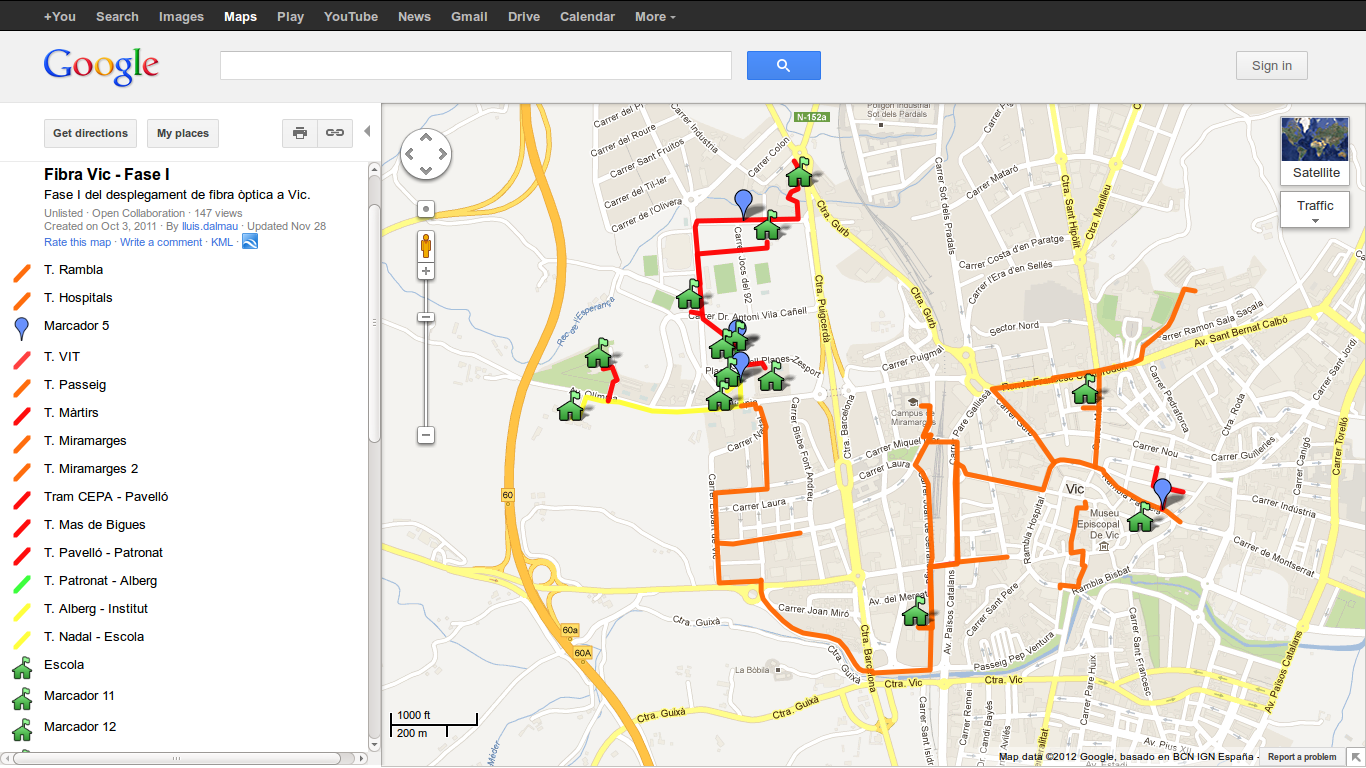
\includegraphics[scale=.33]{sect2/figures/Vic_iteration1.eps} 
  \caption{OF deployment in Vic iteration 1.}
  \label{fig:vic_it1}
\end{figure}


\begin{figure}[htbp]
  \centering
  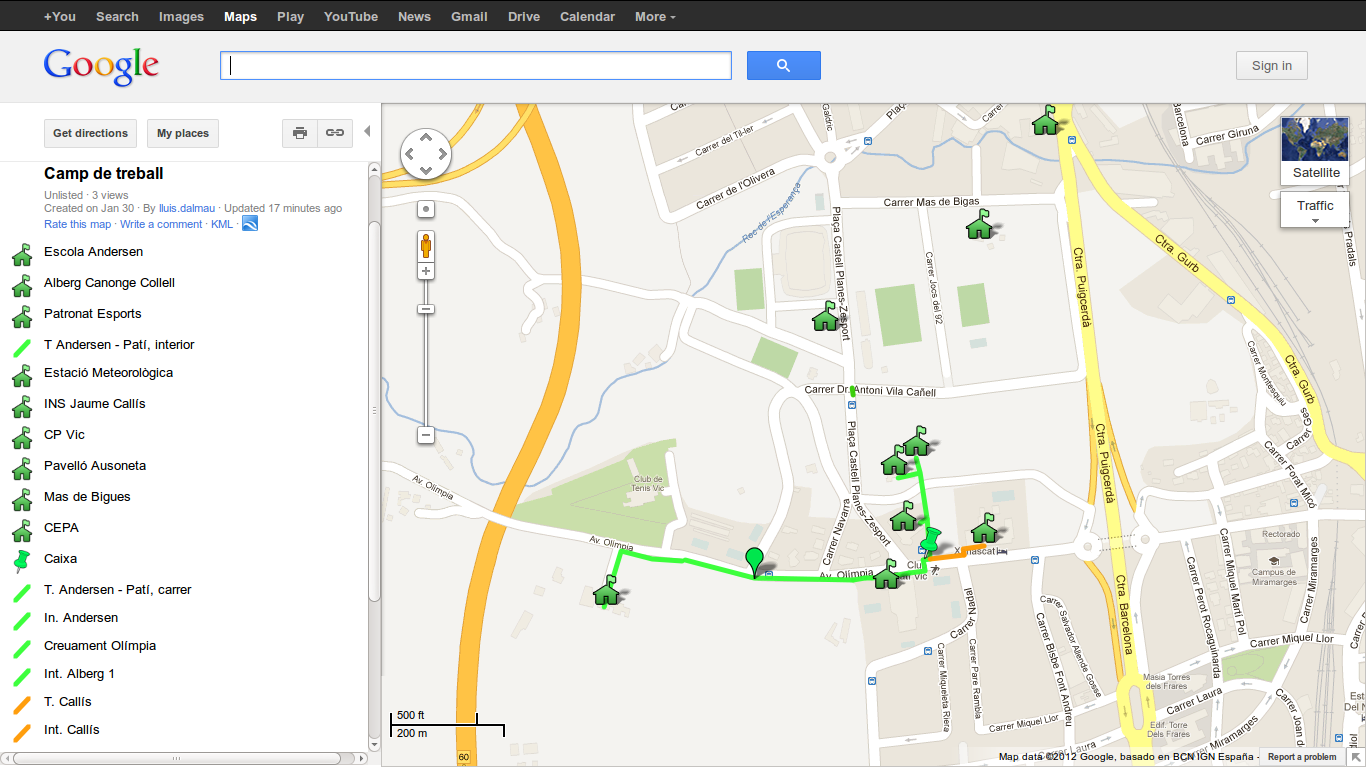
\includegraphics[scale=.33]{sect2/figures/Vic_summer_camp_2012.eps} 
  \caption{OF deployment in Vic iteration 1.}
  \label{fig:vic_sc12}
\end{figure}



\subsubsection{Rub\'{i}}

Rub\'{i} local government in early 2012 showed interest in deploying fiber following a Bottom-up Broadband model.
The first goal was to offer high-speed Internet connections to the largest companies operating in one of Rub\'{i}'s industrial areas called ''Can Jardi''.
These companies had access only to slow ADSL connections and the absence of a fiber deployment was seriously affecting their competitiveness.
The lack of commercial high speed connections offering prompted the city's local government to look for alternatives.

An initial round of conversations took place in Spring 2012 to plan for a deployment during the Summer.
The planning involved a strong participation of a local partner, company with experience in wireless BuB deployment.
This initial planning for a bottom-up-broadband deployment did not pass unnoticed, and commercial ISPs approached the Rub\'{i} local government with fiber deployment offerings.
The offering was to place the city of Rub\'{i} high in de ISPs fiber deployment plans and prioritize it over other cities.
Guifi, UPF and the local partner were asked by the city's local government to prepare a concrete offering that could match the offering of the ISPs.

The arrival of traditional ISPs proposals, combined with the uncertainties of the competence of the local partner to carry out fiber deployments and internal discrepancies in the Rub\'{i}'s local government slowed down the pilot.
Currently this pilot is on hold, and it is not clear how it will resolve.
Personal interests and personal connections within the City Hall may play an important role in the final resolution.

It is remarkable that the fact that the City Hall entered in conversations to plan a BuB deployment triggered a number of events that placed the city in a much favourable situation to negotiate with the ISPs about future fiber deployments.

\subsection{Other deployments}



\section{Points-Of-Presence (POPs)}
\label{sec:POPs}
A Point-Of-Presence (POP) is an artificial demarcation point or interface point between communicating entities. Al POPs mentioned in this documents refers to optical fiber (OF) interconnection points.

Since 2010 the guifi.net community has raised five POPs over the Catalan territory, all of them according to the Bottom-up Broadband (BuB) model specified in the guifi.net network license\footnote{This is the agreement all users must accept to join the network. It's mission is to keep the network free, open and neutral. The Catalan version can be found at \url{http://guifi.net/ca/CXOLN}. It has not yet been translated into English}.
Thus anyone is able to connect to them as long as he/she accepts this license.

From a general perspective guifi.net community is building a set of neutral exchange points, leaving the infrastructure available to the individuals, associations or either companies. These kind of POPs are named POP-IX referring to the Internet eXchange points (IX).

Figure \ref{fig:fibre_map} shows the OF network map of guifi.net POPs as of December 2012. The backbone, i.e. the POPs interconnections are made using third party infrastructures. Currently all the POP interconnection links are over the Xarxa Oberta de Catalunya (XOC)\footnote{\url{http://www.xarxaoberta.cat/en/about-xoc}}.

\begin{figure}[htbp]
  \centering
  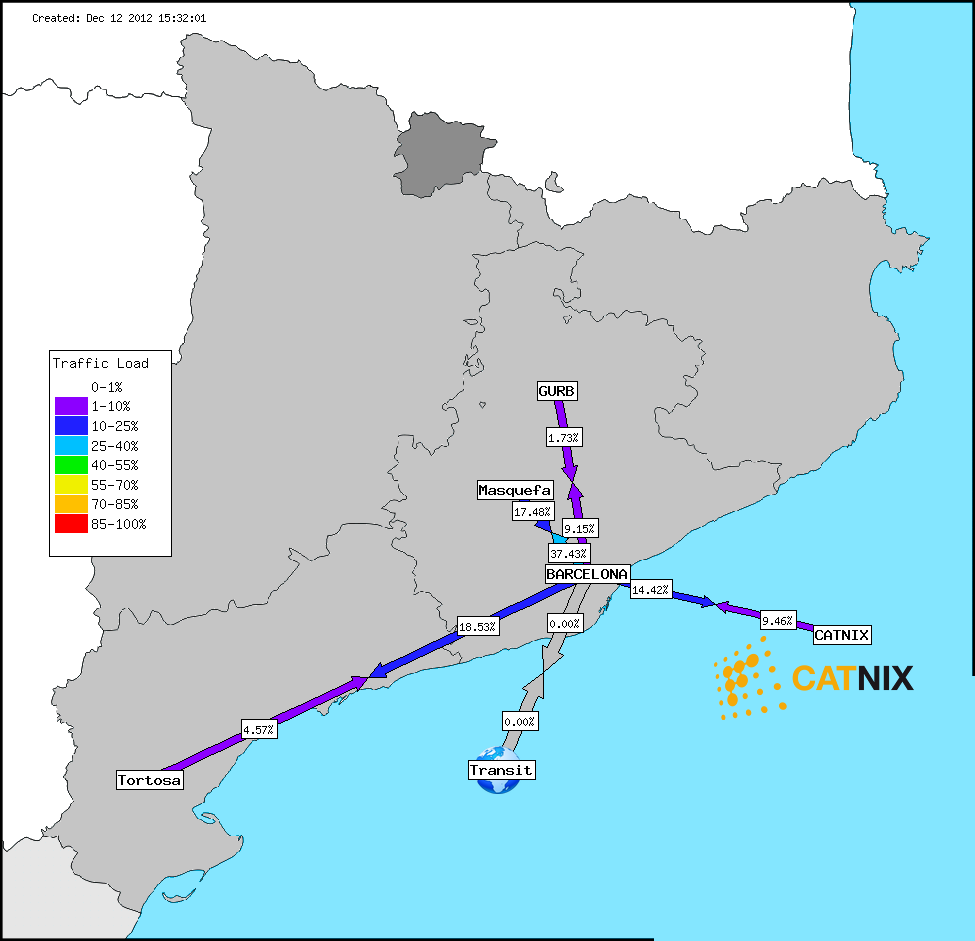
\includegraphics[scale=.35]{pops/figures/pops_network_map.eps} 
  \caption{Guifi.net fiber POPs network map}
  \label{fig:fibre_map}
\end{figure}


\FloatBarrier
\subsection{Pilot's POPs}

\FloatBarrier
\subsubsection{Gurb}
Gurb pilot has its own POP fully operational. The POP is placed in the garage of a home's guifi.net member. The garage also hosts a data center where the guifi.net partners\footnote{A guifi.net partner is a guifi.net member that has professional interest in the network.} can collocate their hardware. Pictures on Figure~\ref{fig:gurb_net_load} shows some details of the current installation.


\begin{figure}[htbp]
  \centering
    \begin{tabular}{cc}
      \resizebox{70mm}{!}{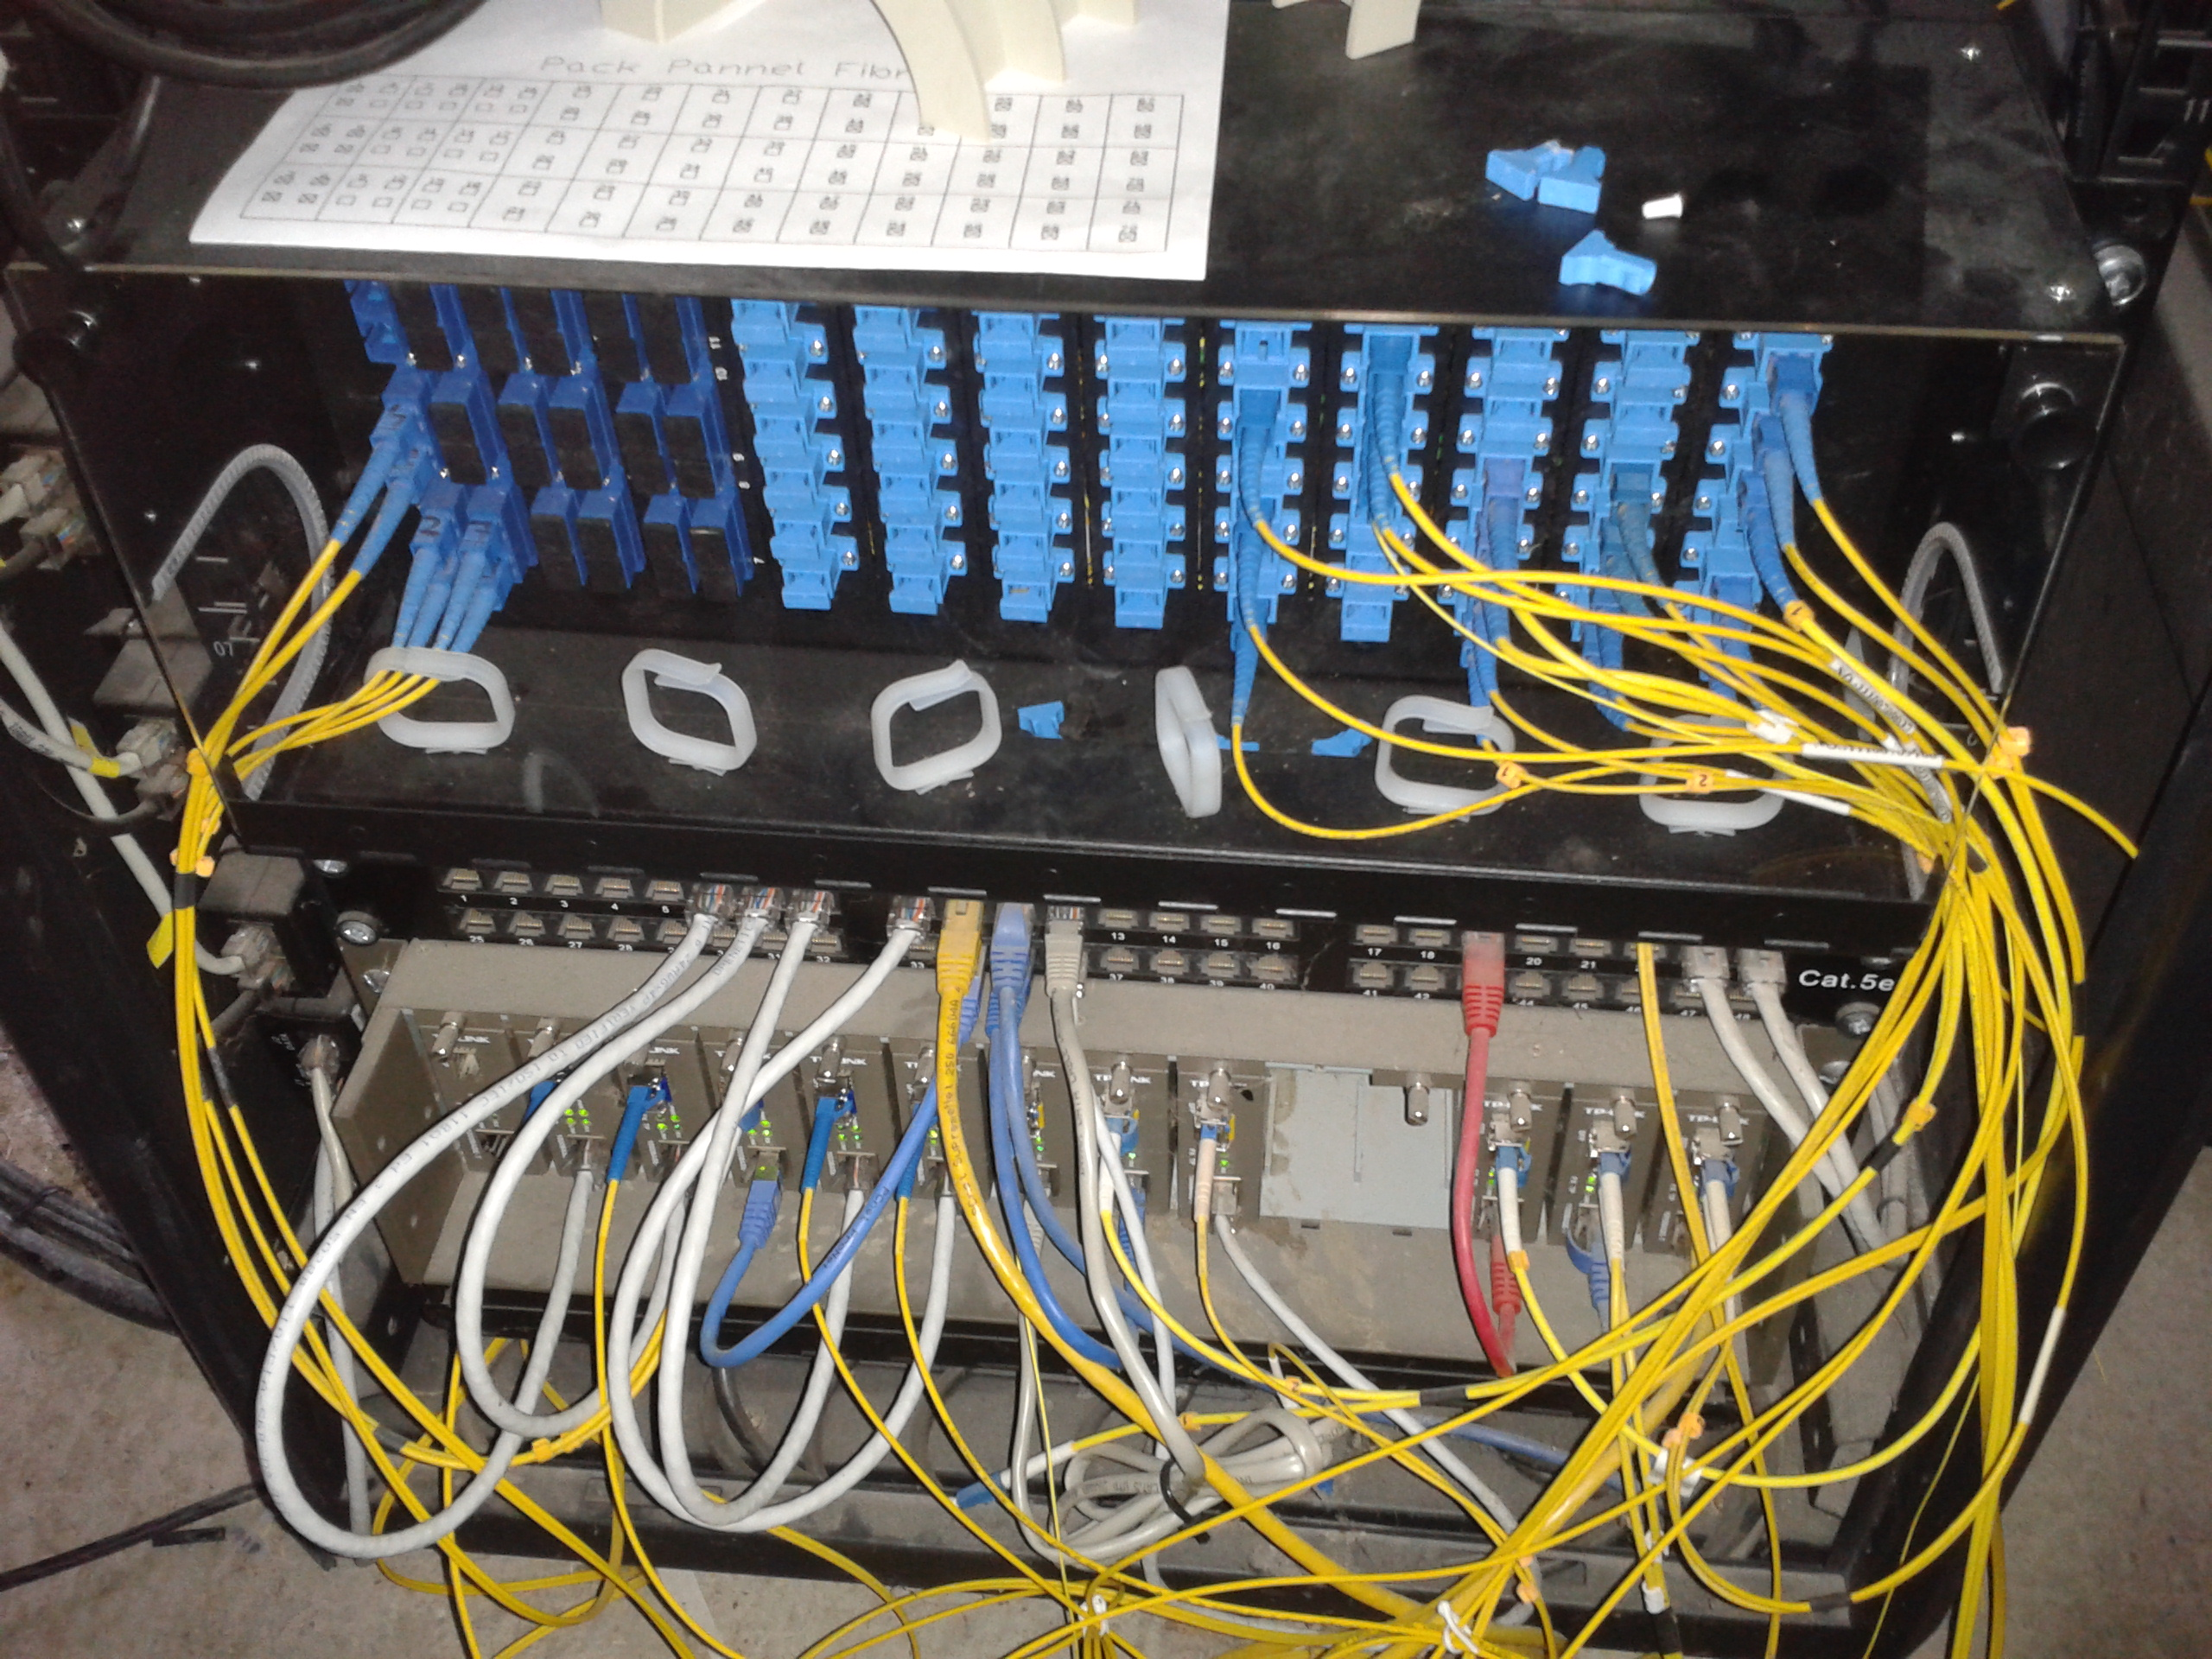
\includegraphics{pops/figures/gurb_rack1.eps}} &
      \resizebox{70mm}{!}{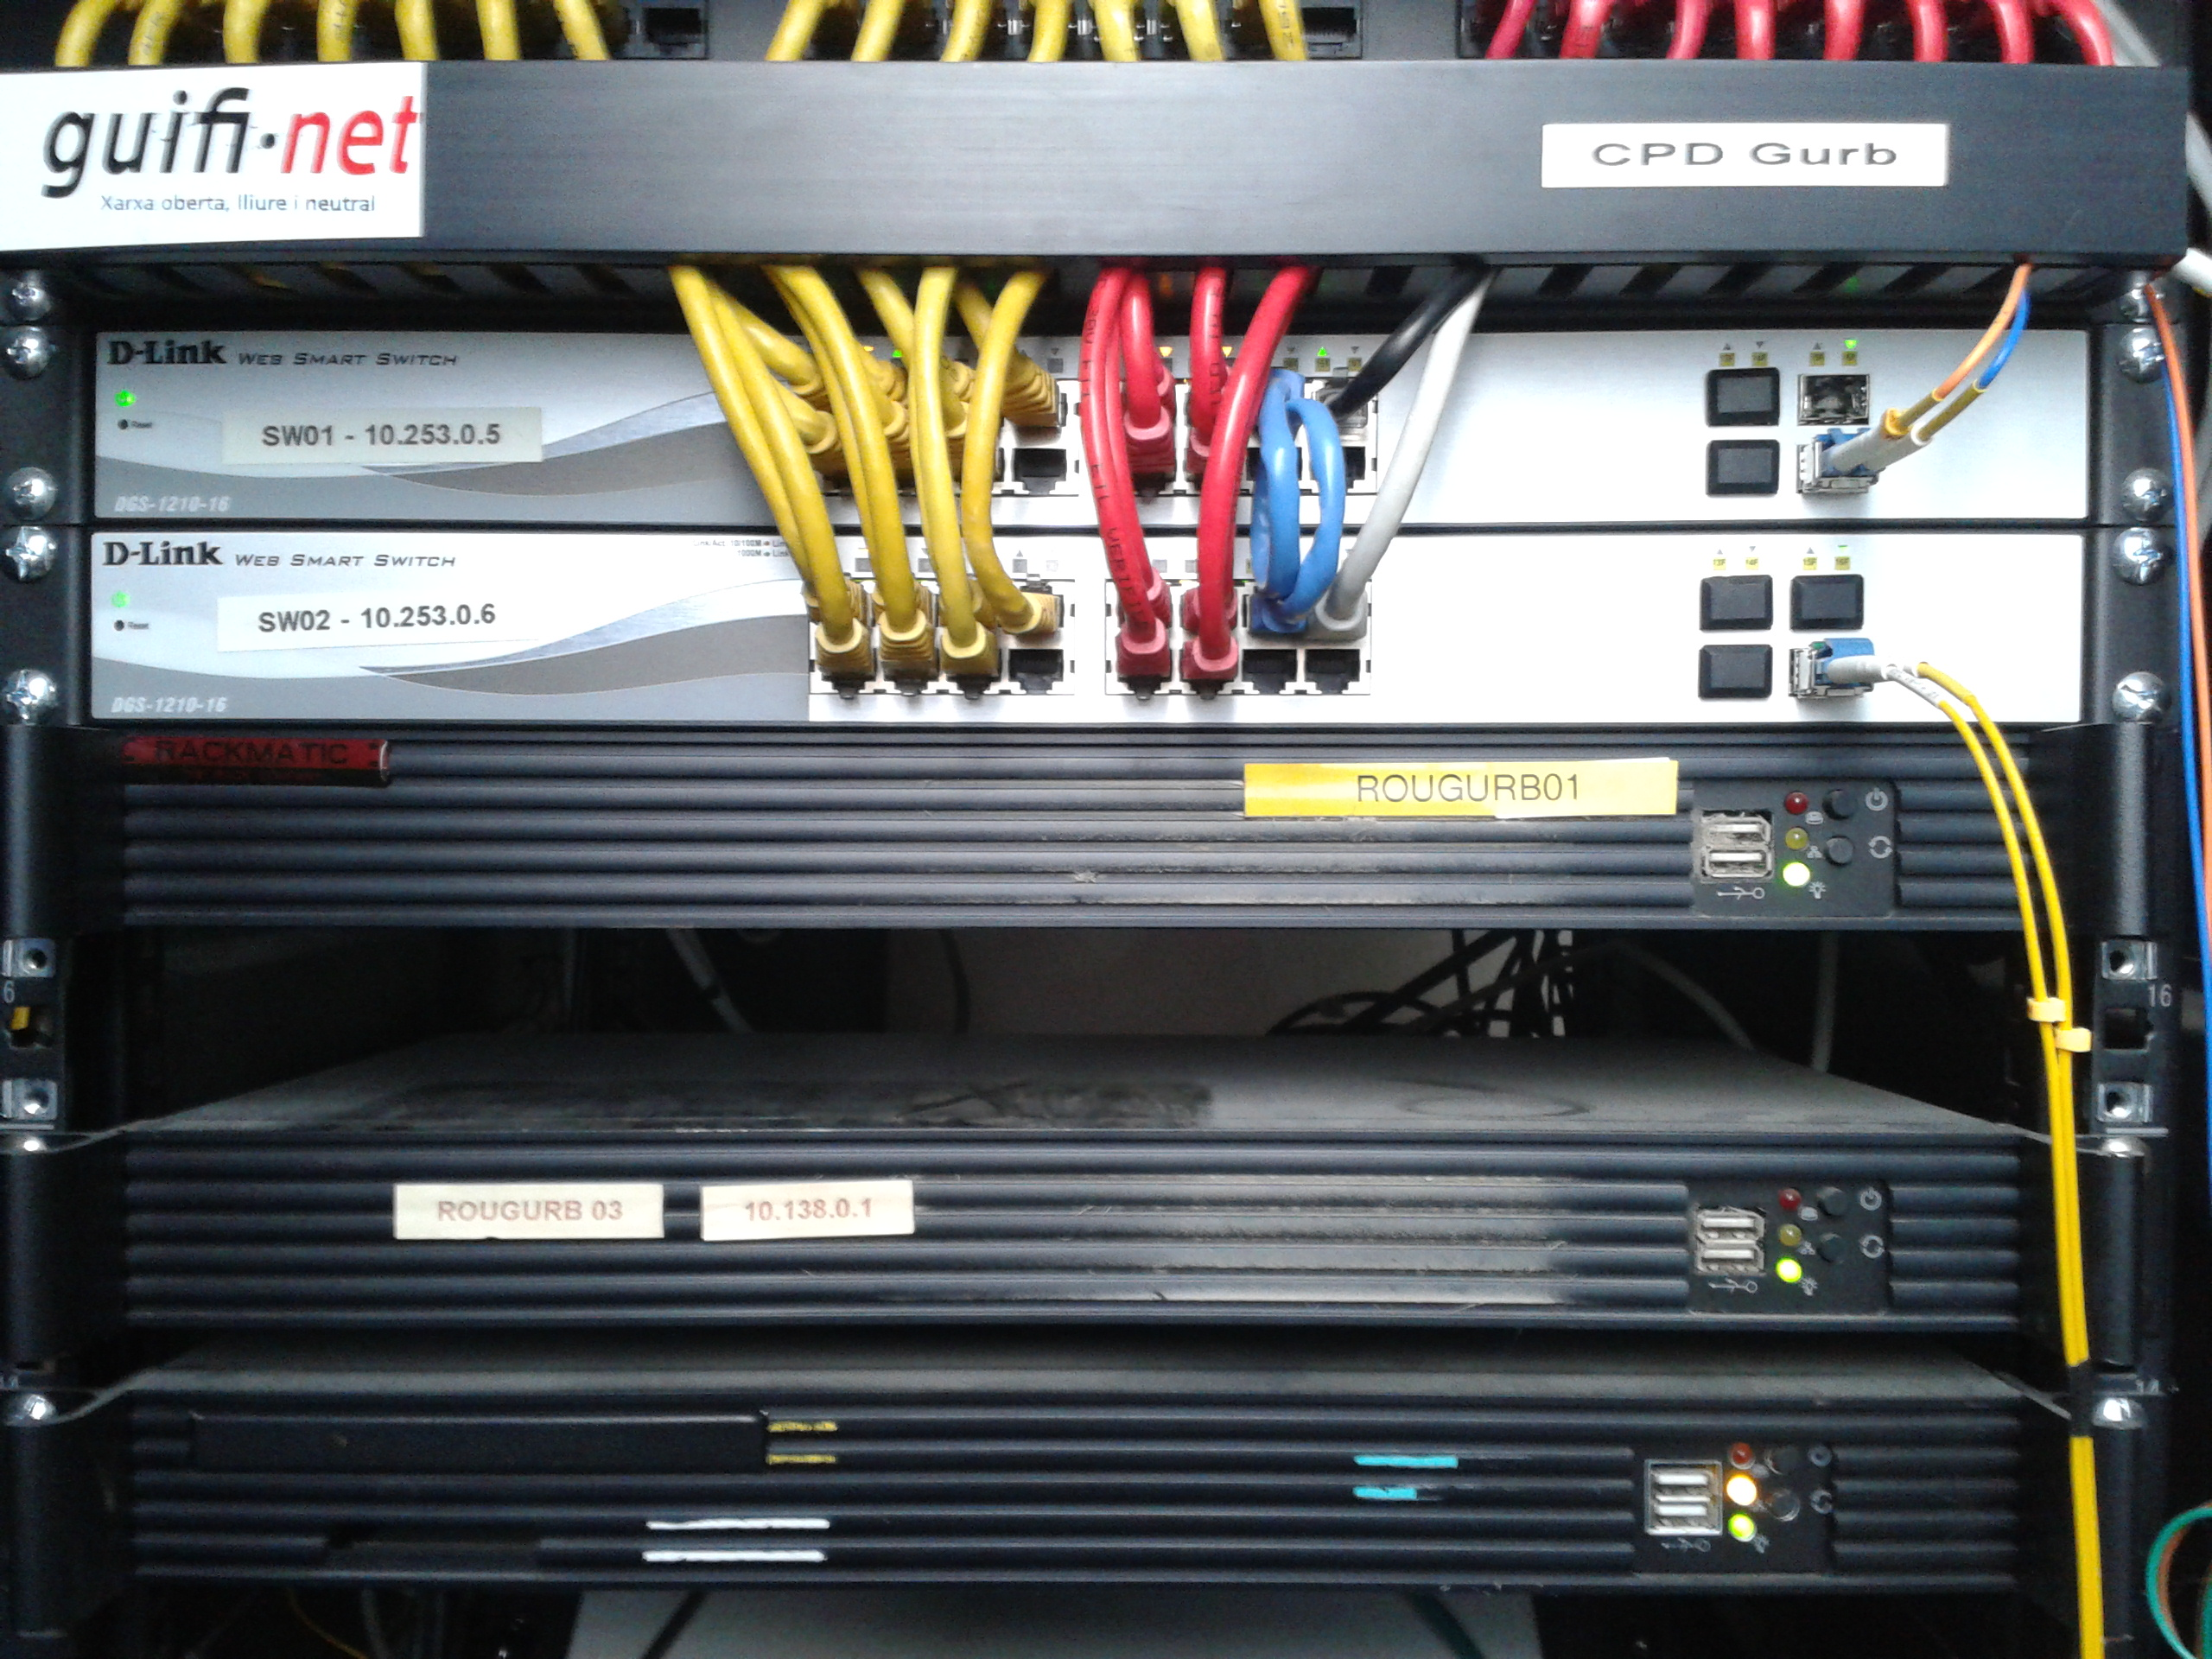
\includegraphics{pops/figures/gurb_rack2.eps}} \\
    \end{tabular}
  \caption{Gurb's POP detailed pictures. On the right the OF terminations. On the left the routers.}
  \label{fig:grub_rack}
\end{figure}

This POP, activated in 2010, was the first one. Figure~\ref{fig:gurb_net_load} shows its traffic load in 2012.

\begin{figure}[htbp]
  \centering
  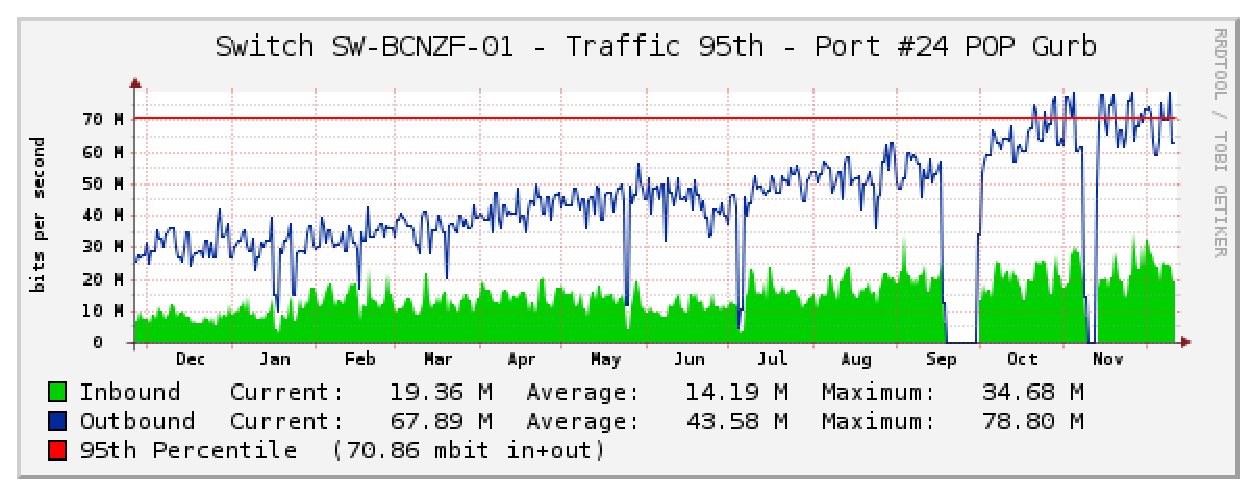
\includegraphics[scale=.65]{pops/figures/gurb_network_load_year.eps} 
  \caption{Gurb's POP network load (year 2012).}
  \label{fig:gurb_net_load}
\end{figure}


\FloatBarrier
\subsubsection{Vic}

The Vic's POP is expected to be fully activated in the coming days.


\FloatBarrier
\subsection{Other POPs}


\FloatBarrier
\subsubsection{Telvent-Barcelona}

Telvent-Barcelona is a commercial data center\footnote{\url{http://www.telvent.es/en/}} placed in an industrial park of Barcelona. It hosts the CATNIX\footnote{\url{http://www.catnix.net}}, the Internet exchange point (IX) of Catalonia, a physical infrastructure provided by the Catalan government. IXs are critical for the Internet since they are meant to let the network operators exchange their information and connect their networks (autonomous systems). 

On the one hand, as be shown in Figure \ref{fig:fibre_map}, all guifi.net POPs are linked to TELVENT-Barcelona. On the other hand, guifi.net connects to the Internet through this POP.

guifi.net Foundation operates it's own backbone infrastructure using the ASN 49835 (Autonomous System Number). 
An open peering policy is followed to establish peering sessions with all potential partners. Figure~\ref{fig:catnix_net_load} shows the total peering traffic of guifi.net CATNIX port\footnote{To be a CATNIX members must have at least one public ASN and one public IP block. Guifi.net is a Local Internet Registry (LIR) since it is a RIPE-NCC member, and has its own ASN numbers and IPv4 and IPv6 blocks.}. Additionally guifi.net Foundation has an Internet Gigabit uplink contracted with Cogent\footnote{\url{http://www.cogentco.com/en/}}. Figure~\ref{fig:cogent_load} . All guifi.net Foundation routers and servers are allocated in a 22U rack in Telvent-Barcelona, shown in Figure~\ref{fig:telvent_rack}. 


Figure \ref{fig:telvent_scheme} shows a connection scheme (layer 2) of the hardware used for the CATNIX POP. 
The first port of the switch SW-03 is the optical fiber which brings the data from the other POPs. As can be seen each
of them use a separate VLAN. The seventh port of the second switch is the connection with the carrier to reach the Internet.
And the eight is connected to the CATNIX infrastructure where the exchange of data with other ISPs and networks is possible. 


The Telvent-Barcelona Foundation resources are shared with other partners, such as puntCat\footnote{\url{http://www.domini.cat/}}, the Catalan Top-Level Domain (TDL), which is currently using half of the space available.

\begin{figure}[htbp]
  \centering
  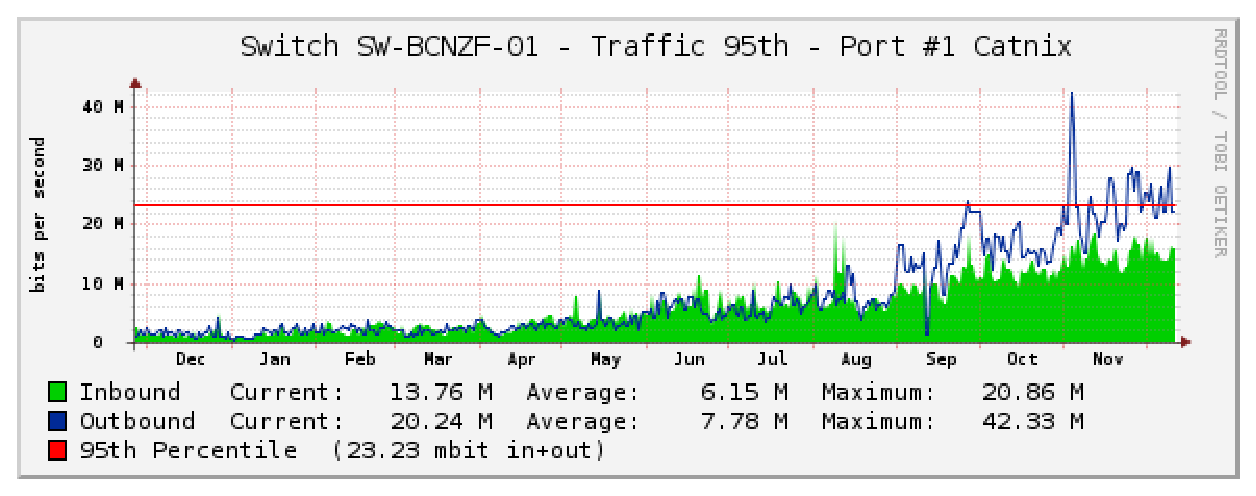
\includegraphics[scale=.65]{pops/figures/catnix_network_load_year.eps} 
  \caption{Telvent-Barcelona's POP network load (year 2012).}
  \label{fig:catnix_net_load}
\end{figure}


\begin{figure}[htbp]
  \centering
  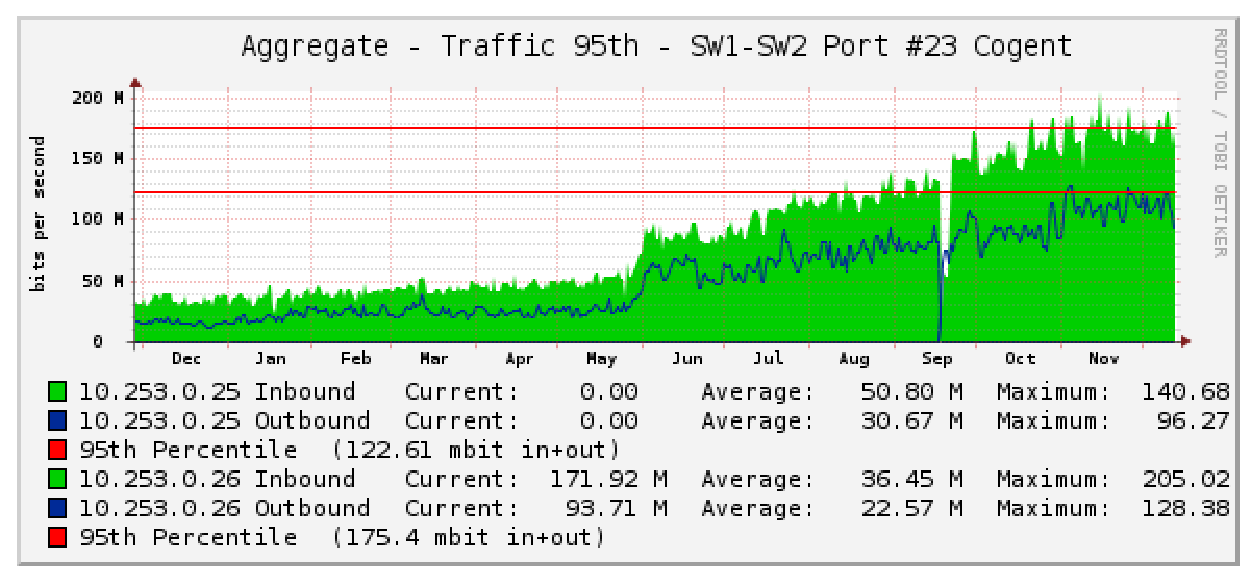
\includegraphics[scale=.65]{pops/figures/cogent_network_load2.eps} 
  \caption{Internet uplink load (year 2012).}
  \label{fig:cogent_load}
\end{figure}


\begin{figure}[htbp]
  \centering
  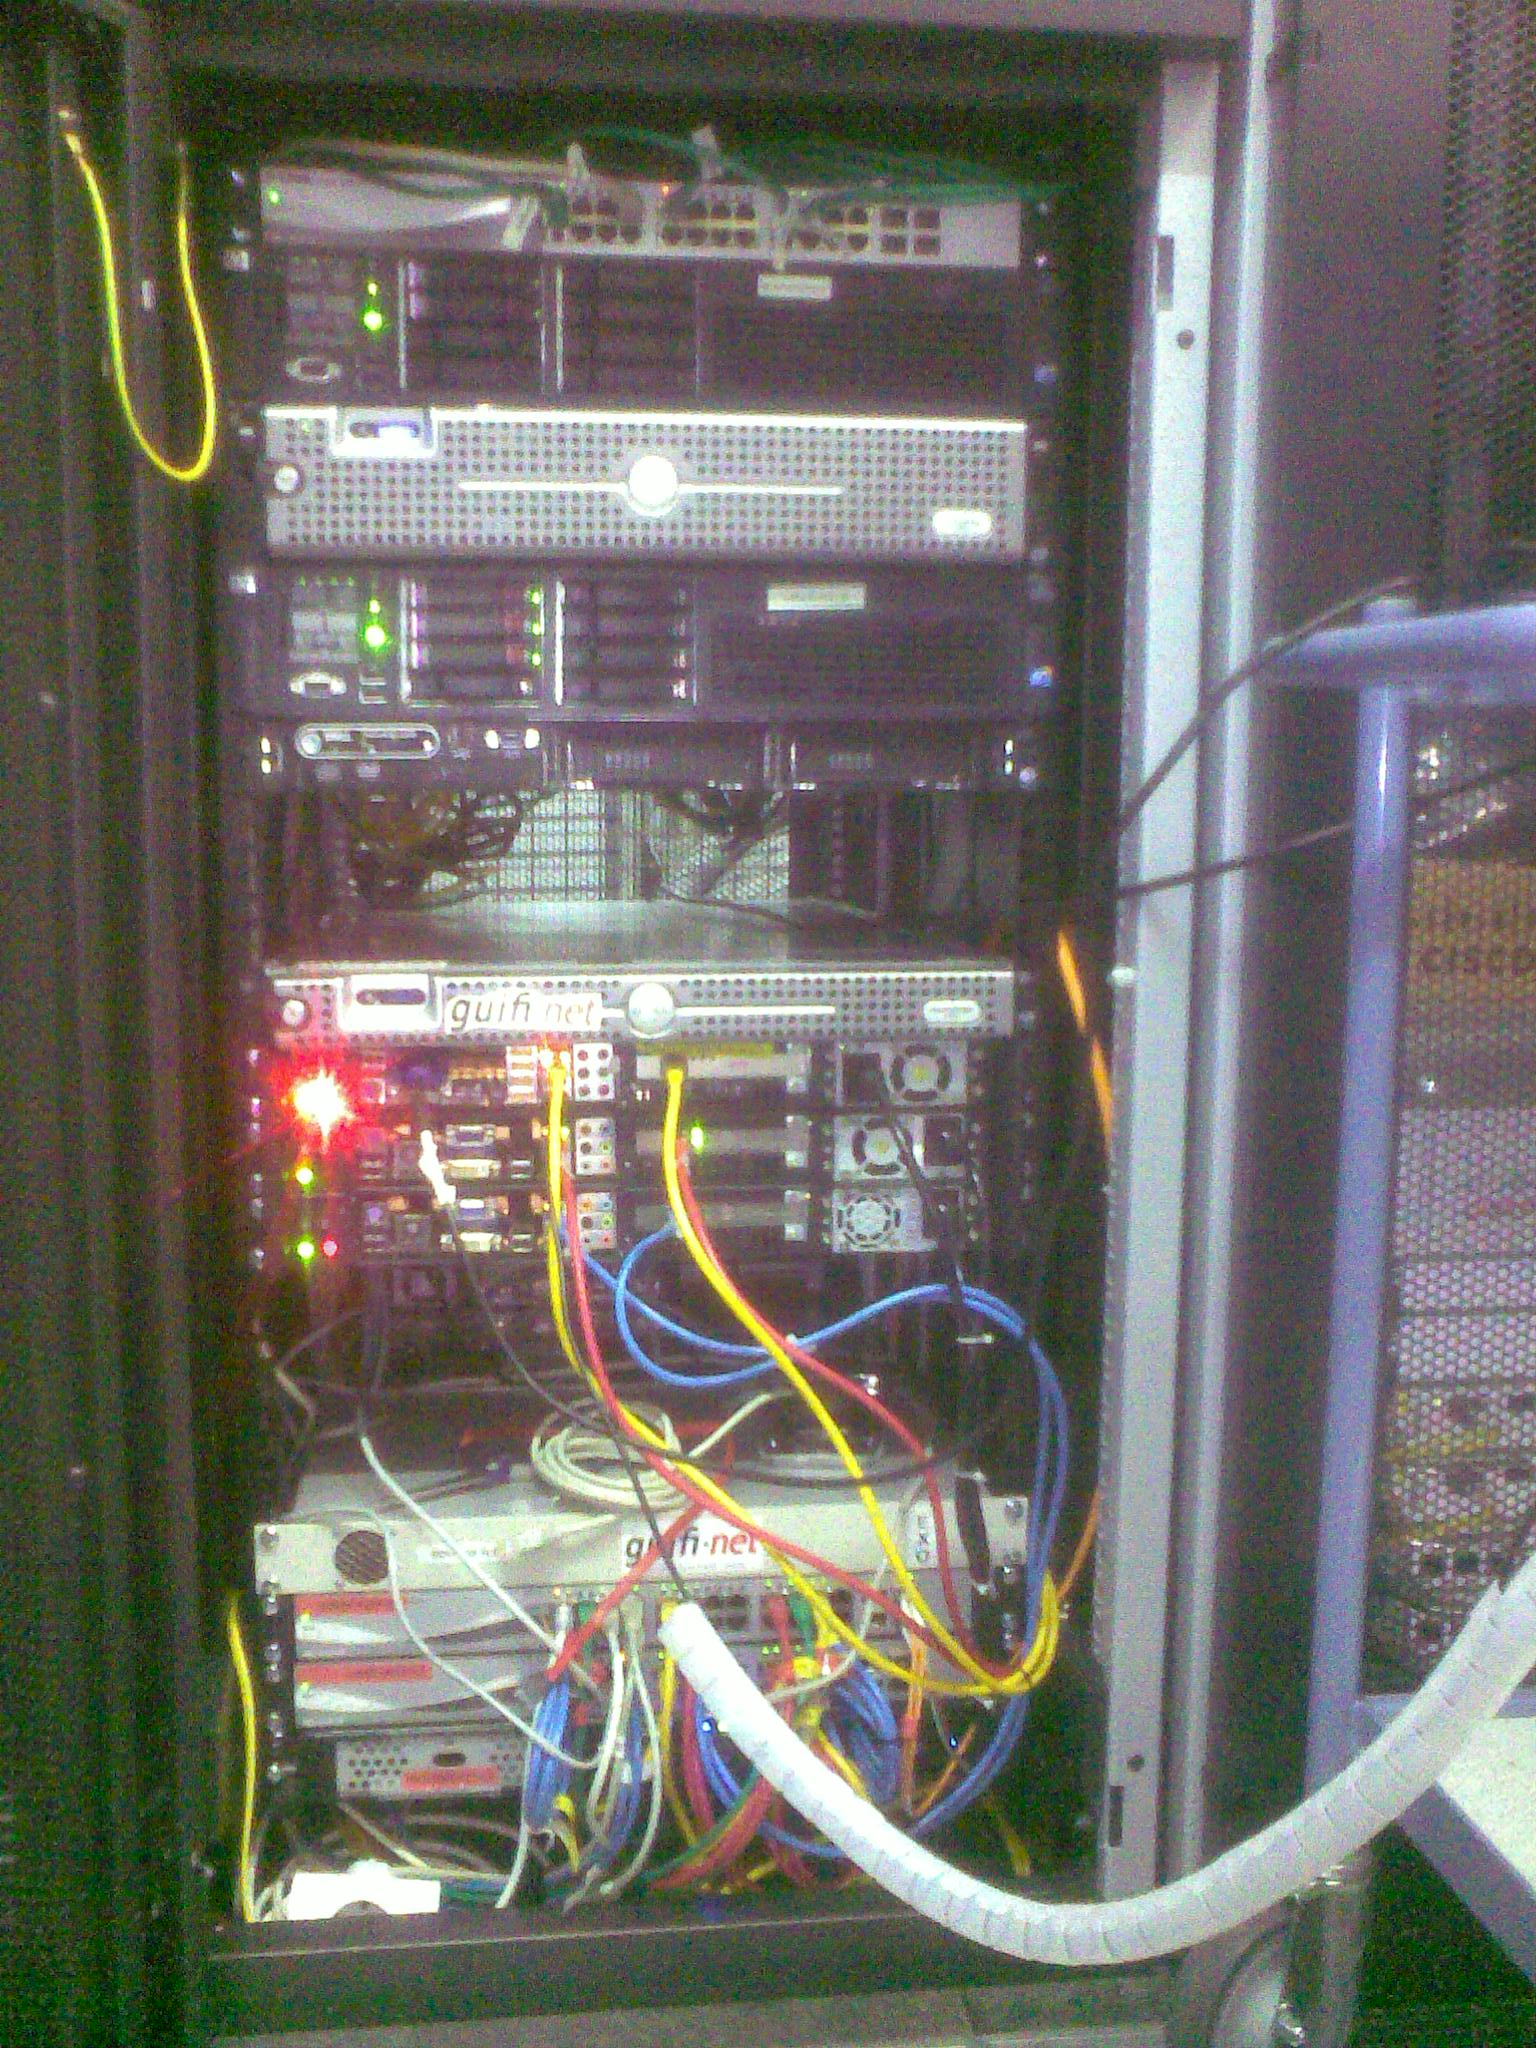
\includegraphics[scale=.65]{pops/figures/telvent_rack_front_view.eps} 
  \caption{guifi.net Foundation rack in TELVENT-Barcelona.}
  \label{fig:telvent_rack}
\end{figure}


\begin{figure}[htbp]
  \centering
  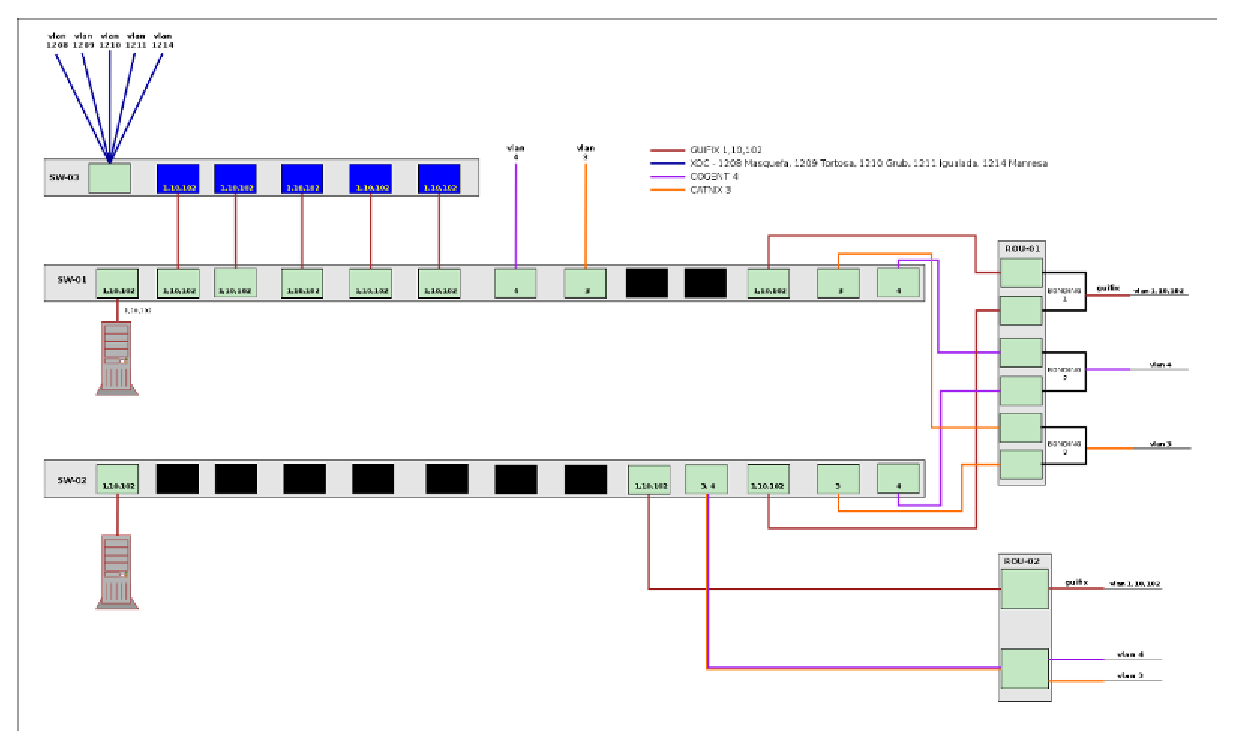
\includegraphics[scale=.75]{pops/figures/telvent_scheme.eps} 
  \caption{CATNIX connections scheme}
  \label{fig:telvent_scheme}
\end{figure}



\FloatBarrier
\subsubsection{Masquefa}

Masquefa is a town of a rural area with a pretty high population density. Due to the poor quality of the Internet access of the traditional telcos the local government undertook a project to bring the broadband to the homes. The project was carried out and is maintained by a local SME. It combines WiFi and OF technologies and integrates a POP which was activated in 2012.

\FloatBarrier
\subsubsection{Igualda}

Igualda is a city similar to Vic. It was one of the pioneers adopting guifi.net outside Osona. The same SME which is operating the Masquefa infrastructure managed to rise a POP in this city also in 2012.


\FloatBarrier
\subsubsection{Tortosa}
Tortosa \footnote{Tortosa, population 34.432 hab, density 157,62 hab/km$^{2}$, the capital of the ''comarca'' of Anoia, Catalonia.} is a city placed on the south of Catalonia. It has a urban center similar to Vic and Igualda but additionaly has a pretty big rural area. The guifi.net users started a project named  OpenFPnet\footnote{\url{http://openfpnet.guifi.net}} with the objective of create an open and neutral fiber backbone around the surrounding villages and set up a POP, which was rised in 2012. From October 2011 to September 2012 the project was partially-funded by the Spanish government through a secondary school\footnote{Institut Montsià, \url{http://www.iesmontsia.org/}}. Currently it is economically sustained by community users grouped in associations and some local SMEs.



\FloatBarrier
\subsubsection{Expected POPs in 2013}

In 2013 other POPs are expected to be risen. The POPs that have a very high probability to happen are:

\begin{itemize}
  \item Balany\`{a}
  \item Centelles
\end{itemize} 

The POPs that can be consolidated during the 2013 are:

\begin{itemize}
  \item Aldea
  \item Matar\'{o}
  \item Cerdanyola
\end{itemize} 


\section{Results}
\label{sec:results}
Figure~\ref{fig:tvChannels} shows the power levels in the collection. Note that the X-axis is labeled with UHF TV channel numbers, each one $8$~MHz-wide and able to contain a maximum of four standard resolution or two high definition TV channels.

One of the tasks of the proposed algorithm~\cite{sanabriaCodeUSRP} is to assign a state (free or occupied) to each channel based on its power readings (in this case, thirty two readings per UHF TV channel). Each channel's state can be identified by looking at the right-hand side Y-axis in Figure~\ref{fig:tvChannels}.

A study performed by Domingo~\emph{et al.}~\cite{domingo2012white}, documented a spectrum sweep with a spectrum analyzer aimed at finding TV White Spaces at the same location as the testings in this work. The presented approach matched nearly 70\% of their observations, revealing 29 TV White Spaces against the 35 observed with the spectrum analyzer. This lower number is possibly due to narrow-band transmissions detected by the USRP.

\begin{figure}[htbp]
  \centering
  \includegraphics[width = 11cm, angle = -90]{sect3/figures/figure1_wo_Albert.eps}
  \caption{USRP-estimated TV White Spaces}
  \label{fig:tvChannels}
\end{figure}


\label{sec:conclusion}
\label{sec:conclusions}
The results of the first year of fiber deployment are outstanding. Firstly, over 60 fiber connections have been made in 2012 (60 farms in the Gurb pilot), and 5 non-residential buildings in the Vic pilot). Secondly, 3 Points-Of-Presence (POPs) have been activated in 2012 and at least 4 expected for 2013, one of a selected pilots (Vic pilot). Thirdly, the activity is not restricted to the selected pilots since many other initiatives are going-on in parallel, some of them very autonomous and barely known by the guifi.net Foundation. Finally, the future is very promising since the model proves to be self-sustainable.

This document is publicly available as a common resource to be shared by the community.



% The very first letter is a 2 line initial drop letter followed
% by the rest of the first word in caps.
% 
% form to use if the first word consists of a single letter:
% \IEEEPARstart{A}{demo} file is ....
% 
% form to use if you need the single drop letter followed by
% normal text (unknown if ever used by IEEE):
% \IEEEPARstart{A}{}demo file is ....
% 
% Some journals put the first two words in caps:
% \IEEEPARstart{T}{his demo} file is ....
% 
% Here we have the typical use of a "T" for an initial drop letter
% and "HIS" in caps to complete the first word.
%\IEEEPARstart{T}{his} is the introduction blah blah blah blah blah blah blah.
%Blah blah blah blah.
%Blah blah blah blah.
%Blah blah blah blah.

% if have a single appendix:
%\appendix[Proof of the Zonklar Equations]
% or
%\appendix  % for no appendix heading
% do not use \section anymore after \appendix, only \section*
% is possibly needed

% use appendices with more than one appendix
% then use \section to start each appendix
% you must declare a \section before using any
% \subsection or using \label (\appendices by itself
% starts a section numbered zero.)
%


%\appendices
%\section{Proof of the First Zonklar Equation}
%Appendix one text goes here.

% you can choose not to have a title for an appendix
% if you want by leaving the argument blank
%\section{}
%Appendix two text goes here.


% use section* for acknowledgement
\section*{Acknowledgment}

This work has been partially funded by the European Commission (grant CIP-ICT PSP-2011-5).
The views expressed in this technical report are solely those of the authors and do not represent the views of the European Commission.


% Can use something like this to put references on a page
% by themselves when using endfloat and the captionsoff option.
%\ifCLASSOPTIONcaptionsoff
%  \newpage
%\fi



% trigger a \newpage just before the given reference
% number - used to balance the columns on the last page
% adjust value as needed - may need to be readjusted if
% the document is modified later
%\IEEEtriggeratref{8}
% The "triggered" command can be changed if desired:
%\IEEEtriggercmd{\enlargethispage{-5in}}

% references section

% can use a bibliography generated by BibTeX as a .bbl file
% BibTeX documentation can be easily obtained at:
% http://www.ctan.org/tex-archive/biblio/bibtex/contrib/doc/
% The IEEEtran BibTeX style support page is at:
% http://www.michaelshell.org/tex/ieeetran/bibtex/
\bibliographystyle{IEEEtran}
% argument is your BibTeX string definitions and bibliography database(s)
\bibliography{IEEEabrv,my_bib}
%
% <OR> manually copy in the resultant .bbl file
% set second argument of \begin to the number of references
% (used to reserve space for the reference number labels box)
%\begin{thebibliography}{1}

%\bibitem{IEEEhowto:kopka}
%H.~Kopka and P.~W. Daly, \emph{A Guide to \LaTeX}, 3rd~ed.\hskip 1em plus
%  0.5em minus 0.4em\relax Harlow, England: Addison-Wesley, 1999.

%\end{thebibliography}

% biography section
% 
% If you have an EPS/PDF photo (graphicx package needed) extra braces are
% needed around the contents of the optional argument to biography to prevent
% the LaTeX parser from getting confused when it sees the complicated
% \includegraphics command within an optional argument. (You could create
% your own custom macro containing the \includegraphics command to make things
% simpler here.)
%\begin{biography}[{\includegraphics[width=1in,height=1.25in,clip,keepaspectratio]{mshell}}]{Michael Shell}
% or if you just want to reserve a space for a photo:

%\begin{IEEEbiography}{Michael Shell}
%Biography text here.
%\end{IEEEbiography}

% if you will not have a photo at all:
%\begin{IEEEbiographynophoto}{John Doe}
%Biography text here.
%\end{IEEEbiographynophoto}

% insert where needed to balance the two columns on the last page with
% biographies
%\newpage

%\begin{IEEEbiographynophoto}{Jane Doe}
%Biography text here.
%\end{IEEEbiographynophoto}

% You can push biographies down or up by placing
% a \vfill before or after them. The appropriate
% use of \vfill depends on what kind of text is
% on the last page and whether or not the columns
% are being equalized.

%\vfill

% Can be used to pull up biographies so that the bottom of the last one
% is flush with the other column.
%\enlargethispage{-5in}



% that's all folks
\end{document}


